\documentclass[tikz,border=5]{standalone}
\usetikzlibrary{automata,arrows,calc,positioning}
\begin{document}
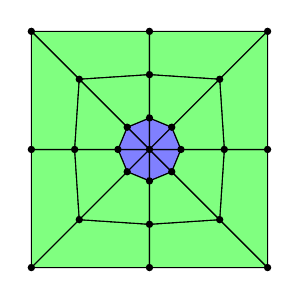
\begin{tikzpicture}[>=stealth', shorten >=1pt, auto,
    node distance=1.5cm, scale=1, 
    transform shape, align=center, 
    state/.style={circle, draw, inner sep=1pt, minimum size=0.0]}]
\coordinate [draw=black,shift={(0,0)}] (0) at (0,0);
\coordinate [draw=black,shift={(0,0)}] (1) at (1.5,0);
\coordinate [draw=black,shift={(0,0)}] (2) at (1.5,1.5);
\coordinate [draw=black,shift={(0,0)}] (3) at (1.5,1.1);
\coordinate [draw=black,shift={(0,0)}] (4) at (1.2171572876,1.2171572876);
\coordinate [draw=black,shift={(0,0)}] (5) at (1.1,1.5);
\coordinate [draw=black,shift={(0,0)}] (6) at (0,1.5);
\coordinate [draw=black,shift={(0,0)}] (7) at (0,3);
\coordinate [draw=black,shift={(0,0)}] (8) at (1.2171572876,1.7828427124);
\coordinate [draw=black,shift={(0,0)}] (9) at (1.5,1.9);
\coordinate [draw=black,shift={(0,0)}] (10) at (1.5,3);
\coordinate [draw=black,shift={(0,0)}] (11) at (3,0);
\coordinate [draw=black,shift={(0,0)}] (12) at (1.7828427124,1.2171572876);
\coordinate [draw=black,shift={(0,0)}] (13) at (1.9,1.5);
\coordinate [draw=black,shift={(0,0)}] (14) at (3,1.5);
\coordinate [draw=black,shift={(0,0)}] (15) at (3,3);
\coordinate [draw=black,shift={(0,0)}] (16) at (1.7828427124,1.7828427124);
\coordinate [draw=black,shift={(0,0)}] (17) at (1.5,0.5500000000014312);
\coordinate [draw=black,shift={(0,0)}] (18) at (0.6085786437983935,0.6085786437983935);
\coordinate [draw=black,shift={(0,0)}] (19) at (0.5500000000014312,1.5);
\coordinate [draw=black,shift={(0,0)}] (20) at (0.6085786437983723,2.391421356201628);
\coordinate [draw=black,shift={(0,0)}] (21) at (1.5,2.449999999998004);
\coordinate [draw=black,shift={(0,0)}] (22) at (2.391421356201628,0.6085786437983723);
\coordinate [draw=black,shift={(0,0)}] (23) at (2.449999999998004,1.5);
\coordinate [draw=black,shift={(0,0)}] (24) at (2.391421356201648,2.391421356201648);
\draw [fill=blue!50] (2) --  (4) --  (3) -- cycle;
\draw [fill=blue!50] (2) --  (4) --  (5) -- cycle;
\draw [fill=blue!50] (2) --  (8) --  (9) -- cycle;
\draw [fill=blue!50] (2) --  (8) --  (5) -- cycle;
\draw [fill=blue!50] (2) --  (12) --  (3) -- cycle;
\draw [fill=blue!50] (2) --  (12) --  (13) -- cycle;
\draw [fill=blue!50] (2) --  (16) --  (9) -- cycle;
\draw [fill=blue!50] (2) --  (16) --  (13) -- cycle;
\draw [fill=green!50] (0) --  (18) --  (17) --  (1) -- cycle;
\draw [fill=green!50] (18) --  (4) --  (3) --  (17) -- cycle;
\draw [fill=green!50] (0) --  (18) --  (19) --  (6) -- cycle;
\draw [fill=green!50] (18) --  (4) --  (5) --  (19) -- cycle;
\draw [fill=green!50] (7) --  (20) --  (21) --  (10) -- cycle;
\draw [fill=green!50] (20) --  (8) --  (9) --  (21) -- cycle;
\draw [fill=green!50] (7) --  (20) --  (19) --  (6) -- cycle;
\draw [fill=green!50] (20) --  (8) --  (5) --  (19) -- cycle;
\draw [fill=green!50] (11) --  (22) --  (17) --  (1) -- cycle;
\draw [fill=green!50] (22) --  (12) --  (3) --  (17) -- cycle;
\draw [fill=green!50] (11) --  (22) --  (23) --  (14) -- cycle;
\draw [fill=green!50] (22) --  (12) --  (13) --  (23) -- cycle;
\draw [fill=green!50] (15) --  (24) --  (21) --  (10) -- cycle;
\draw [fill=green!50] (24) --  (16) --  (9) --  (21) -- cycle;
\draw [fill=green!50] (15) --  (24) --  (23) --  (14) -- cycle;
\draw [fill=green!50] (24) --  (16) --  (13) --  (23) -- cycle;
\node [fill=black, draw=none, circle, inner sep=0pt, minimum size=0.1cm,scale=0.3] at (0) {h};
\node [fill=black, draw=none, circle, inner sep=0pt, minimum size=0.1cm,scale=0.3] at (1) {h};
\node [fill=black, draw=none, circle, inner sep=0pt, minimum size=0.1cm,scale=0.3] at (2) {h};
\node [fill=black, draw=none, circle, inner sep=0pt, minimum size=0.1cm,scale=0.3] at (3) {h};
\node [fill=black, draw=none, circle, inner sep=0pt, minimum size=0.1cm,scale=0.3] at (4) {h};
\node [fill=black, draw=none, circle, inner sep=0pt, minimum size=0.1cm,scale=0.3] at (5) {h};
\node [fill=black, draw=none, circle, inner sep=0pt, minimum size=0.1cm,scale=0.3] at (6) {h};
\node [fill=black, draw=none, circle, inner sep=0pt, minimum size=0.1cm,scale=0.3] at (7) {h};
\node [fill=black, draw=none, circle, inner sep=0pt, minimum size=0.1cm,scale=0.3] at (8) {h};
\node [fill=black, draw=none, circle, inner sep=0pt, minimum size=0.1cm,scale=0.3] at (9) {h};
\node [fill=black, draw=none, circle, inner sep=0pt, minimum size=0.1cm,scale=0.3] at (10) {h};
\node [fill=black, draw=none, circle, inner sep=0pt, minimum size=0.1cm,scale=0.3] at (11) {h};
\node [fill=black, draw=none, circle, inner sep=0pt, minimum size=0.1cm,scale=0.3] at (12) {h};
\node [fill=black, draw=none, circle, inner sep=0pt, minimum size=0.1cm,scale=0.3] at (13) {h};
\node [fill=black, draw=none, circle, inner sep=0pt, minimum size=0.1cm,scale=0.3] at (14) {h};
\node [fill=black, draw=none, circle, inner sep=0pt, minimum size=0.1cm,scale=0.3] at (15) {h};
\node [fill=black, draw=none, circle, inner sep=0pt, minimum size=0.1cm,scale=0.3] at (16) {h};
\node [fill=black, draw=none, circle, inner sep=0pt, minimum size=0.1cm,scale=0.3] at (17) {h};
\node [fill=black, draw=none, circle, inner sep=0pt, minimum size=0.1cm,scale=0.3] at (18) {h};
\node [fill=black, draw=none, circle, inner sep=0pt, minimum size=0.1cm,scale=0.3] at (19) {h};
\node [fill=black, draw=none, circle, inner sep=0pt, minimum size=0.1cm,scale=0.3] at (20) {h};
\node [fill=black, draw=none, circle, inner sep=0pt, minimum size=0.1cm,scale=0.3] at (21) {h};
\node [fill=black, draw=none, circle, inner sep=0pt, minimum size=0.1cm,scale=0.3] at (22) {h};
\node [fill=black, draw=none, circle, inner sep=0pt, minimum size=0.1cm,scale=0.3] at (23) {h};
\node [fill=black, draw=none, circle, inner sep=0pt, minimum size=0.1cm,scale=0.3] at (24) {h};
\end{tikzpicture}
\end{document}
